\documentclass[assignment02_Solutions]{subfiles}

\IfSubStr{\jobname}{\detokenize{Solutions}}{\toggletrue{solutions}}{\togglefalse{solutions}}

\fancypagestyle{firstpage}

{\rhead{Assignment 2 \linebreak \textit{Version: \today}}}

\title{Assignment 2: Probabilistic Graphical Models}
\author{Machine Learning}
\date{Fall 2019}

\begin{document}

\maketitle
\thispagestyle{firstpage}


\begin{learningobjectives}
\bi
\item TODO
\ei
\end{learningobjectives}

\section{Motivation and Context}
\bi
\item We’ve learned how probabilities can be used to describe uncertainty in the world
\item We’ve learned how Bayes' rule can be used to reason about hypotheses, models, or other things that cannot be directly observed.
\ei

\section{Product Rule and Marginalization for Random Variables}
\begin{recall}[Product Rule and Marginalization for Events]
Last assignment we learned about two very powerful techniques for computing the probability of events.
\bi
\item The first technique we learned was the product rule (or conjunction rule), which states that for any two events $\mathcal{A}$ and $\mathcal{B}$,
\begin{align}
p(\mathcal{A}, \mathcal{B}) &= p(\mathcal{A}) p(\mathcal{B}|\mathcal{A}) \\
&= p(\mathcal{B}) p(\mathcal{A}|\mathcal{B}) \enspace  . \nonumber
\end{align}
\item The second technique we learned was marginalization.  This technique states that for any two events $\mathcal{A}$ and $\mathcal{B}$,
\begin{align}
p(\mathcal{A}) &= p(\mathcal{A}, \mathcal{B}) + p(\mathcal{A}, \neg \mathcal{B})
\end{align}
\ei
\end{recall}

It turns out that these rules can be applied to 

\section{Conditional Independence of Random Variables}



\section{Bayesian Networks}

\subsection{Simple Example}

\begin{center}
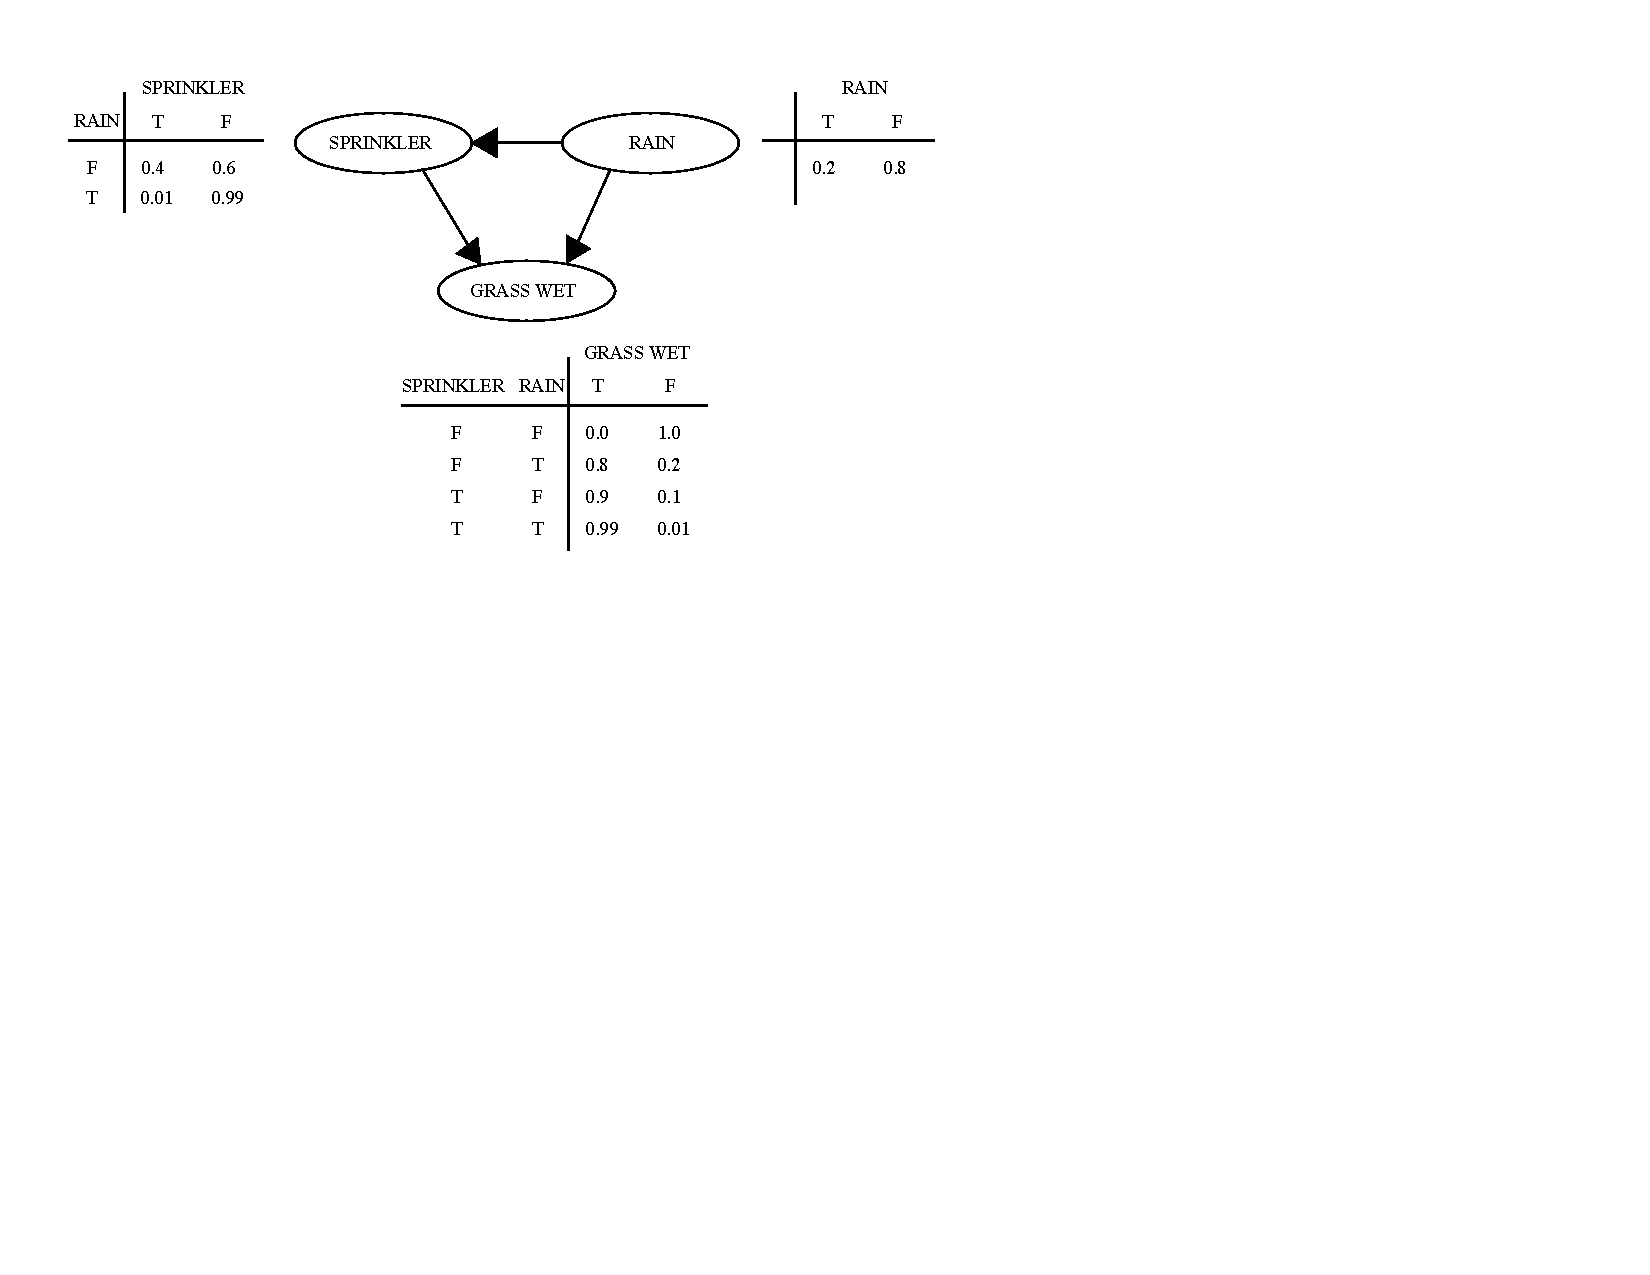
\includegraphics[width=0.7\linewidth]{figures/SimpleBayesNet}
\end{center}

\bi
\item Link to external resources
\item D-separation
\begin{externalresources}
\bi
\item Read \href{http://bayes.cs.ucla.edu/BOOK-09/ch11-1-2-final.pdf}{d-Separation without Tears}.
\item \href{https://www.youtube.com/watch?v=yDs_q6jKHb0}{Pieter Abbeel Lecture} (not sure how clear this is)
\item \href{https://www.youtube.com/watch?v=IjoWqnH6HmU}{This one seems pretty good}
\ei
\end{externalresources}
\item State the main conditions
\item Do some exercises to determine when things are conditionally independent
\ei

\begin{exercise}
The alarm problem (need to find this one from CSE250A) (\href{http://aima.eecs.berkeley.edu/slides-pdf/chapter14a.pdf}{This has the description of the same network}).  \href{https://people.cs.pitt.edu/~milos/courses/cs2740/Lectures/class19.pdf}{More detail on the same network}.
\end{exercise}

\section{Generative versus Discriminative Models}
TODO: write some intro here

\subsection{Discriminative Models: a Look Back at Logistic Regression}

Let's take a minute and think back to the logistic regression model for binary classification that we learned about in module 1.  Given an input point $\mathbf{x_i}$, the logistic regression utilized a weight vector $\mathbf{w}$ to compute the probability that the corresponding output $y_i$ was 1 using the $\sigma(\mathbf{w}^\top \mathbf{x_i}) = \frac{1}{1+e^{-\mathbf{w}^\top \mathbf{x_i}}}$ (recall that $\sigma$ is known as the sigmoid function and serves to squash its input into a number between 0 and 1, which can serve as a valid probability).  While we didn't quite have the vocabulary for it then, what we really doing at the time was computing a conditional probability.  We can think of $Y_i$ as a random variable that represents the output that corresponds to the the input point $\mathbf{x_i}$ ($Y_i$ is either 0 or 1 since we are dealing with binary classification).  We can also think of the input as a random variable $\mathbf{X_i}$ (thinking of the input in this way will be helpful later in this section).  In this way, we can think of what the logistic regression algorithm is doing as computing the following conditional probability:
\begin{align}
p(Y_i = 1 | X_i = \mathbf{x_i}) &= \sigma(\mathbf{w}^\top \mathbf{x_i}) \enspace .
\end{align}

We then defined a loss function that would let us find the best weights, $\mathbf{w}$, given a training set of corresponding input output pairs $(\mathbf{x_1}, y_1), (\mathbf{x_2}, y_2), \ldots, (\mathbf{x_n}, y_n)$.  The details of how we did this are not important to the point we are trying to make now, so it'll suffice to say that learning in a logistic regression model meant tuning the conditional distribution of the outputs (the $Y_i$'s) given the inputs ($\mathbf{x_i}$'s) to fit the training data the best.  This type of model is what is known as a \emph{discriminative model} (the \href{https://en.wikipedia.org/wiki/Discriminative_model}{Wikipedia article on discriminative models} has more details if you are interested).


\begin{understandingcheck}
TODO
\end{understandingcheck}

\subsection{Generative Models}
While the approach outlined above is totally logical, it is not the only way to approach supervised machine learning.  Using a simple application of Bayes' rule, we can derive a whole new approach to the problem!  Since we are interested in predicting $Y_i$ given some inputs $\mathbf{x_i}$ it of course makes sense, for example for a binary classification problem, to want to determine $p(Y_i = 1 | \mathbf{x_i})$.  Instead of modeling that distribution directly, we can instead use Bayes' rule to transform this probability distribution.

TODO: not sure if we should introduce a convention along the lines of $p(\mathbf{x_i}) = p(X_i = \mathbf{x_i})$.

\begin{align}
p(Y_i  = 1 | X_i = \mathbf{x_i}) &= \frac{p(X_i = \mathbf{x_i} | Y_i = 1) p(Y_i = 1)}{p(X_i = \mathbf{x_i})} \label{eq:pgm} \\
&= \frac{p(X_i = \mathbf{x_i} | Y_i = 1) p(Y_i = 1)}{p(X_i =  \mathbf{x_i} | Y_i = 1) p(Y_i = 1) + p(X_i = \mathbf{x_i} | Y_i = 0) p(Y_i = 0)} \nonumber
\end{align}

\begin{marginfigure}
\begin{center}
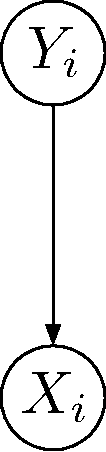
\includegraphics[width=0.2\linewidth]{figures/pgm}
\end{center}
\caption{The graphical model corresponding to a probabilistic generative model in which the latent variable $Y_i$ is thought of as a causally generating $X_i$.\label{fig:pgm}}
\end{marginfigure}

What these equations are telling us is that if we have a model of the probability of the output being 1 \emph{a priori} ($p(Y_i = 1)$) along with a model of the inputs $\mathbf{x_i}$ given the output $Y_i$ ($p(Y_i | \mathbf{x_i})$), then we have all the information we need to compute $p(Y_i = 1 | \mathbf{x}_i)$.  In a way this amounts to adopting the perspective that the hidden output $Y_i$ causes the input $X_i$ (see Figure~\ref{fig:pgm}).

The natural question you might ask yourself is \emph{why?} Here are some potential advantages of using probabilistic generative models.
\bi
\item Suppose you found out that $p(Y_i = 1)$ changed for some reason (any thoughts on when this might happen?  Post here on NB).  Incorporating this change into a probabilistic graphical model would be very straight forward (just modify $p(Y_i =1)$ in Equation~\ref{eq:pgm}).
\ei

\begin{understandingcheck}
TODO
\end{understandingcheck}


\section{Your First Generative Model: Na\"ive Bayes}
\begin{marginfigure}
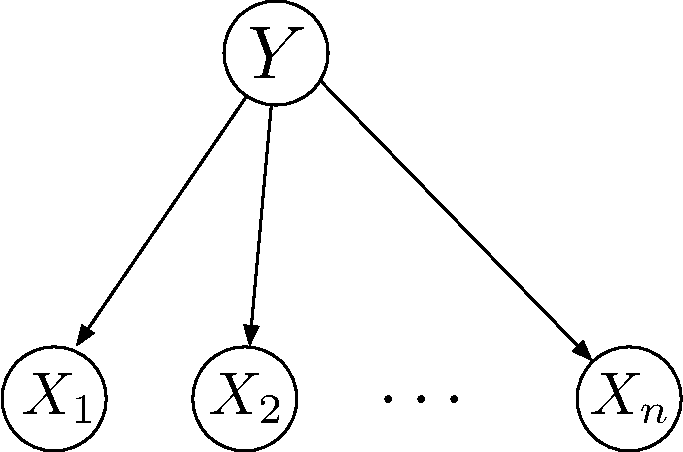
\includegraphics[width=\linewidth]{figures/naivebayesgm}
\end{marginfigure}



\section{Probabilistic frameworks for Fairness in ML}

\section{Compas Model of Recidivism}


\end{document}
